
The Partition Coloring Problem (PCP) is a generalization of the Standard Vertex Coloring Problem (VCP) and has initially been considered by Li and Simha in \cite{li-00}. The problem arose from considering the join problem of routing and wavelength assignment in Wavelength Division Multiplexing optical networks. It is therefore a subproblem of a variant of the Wavelength Routing and Assignment Problem (RWA), namely the min-RWA problem. This chapter aims to give formal definitions and examples of VCP, PCP and min-RWA and reasons about their computational complexities.

\section{Standard Vertex Coloring Problem}
As this thesis refers to VCP in various contexts and for the sake of completeness, this section provides a formal definition, although the problem has already been explained as an example in chapter \ref{ch:prelim}. \\
Given a non-directed graph $G=(V,E)$, the VCP consists in assigning a color to each node in $V$, such that no adjacent nodes have the same color. The aim is to minimize the chromatic number, i.e. the total number of colors used. Figure \ref{pd:vcp} shows a simple graph colored with three colors.

\begin{figure}
\begin{center}

\ifx\du\undefined
  \newlength{\du}
\fi
\setlength{\du}{15\unitlength}
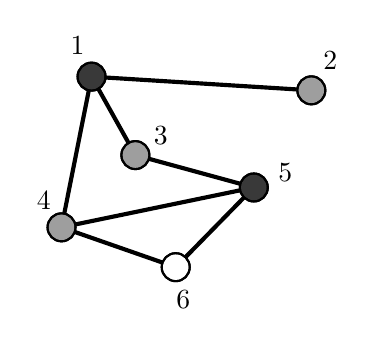
\begin{tikzpicture}[scale=0.6]
\pgftransformxscale{1.000000}
\pgftransformyscale{-1.000000}
\definecolor{dialinecolor}{rgb}{0.000000, 0.000000, 0.000000}
\pgfsetstrokecolor{dialinecolor}
\definecolor{dialinecolor}{rgb}{1.000000, 1.000000, 1.000000}
\pgfsetfillcolor{dialinecolor}
\pgfsetlinewidth{0.050000\du}
\pgfsetdash{}{0pt}
\pgfsetdash{}{0pt}
\pgfsetbuttcap
\pgfsetmiterjoin
\pgfsetlinewidth{0.050000\du}
\pgfsetbuttcap
\pgfsetmiterjoin
\pgfsetdash{}{0pt}
\definecolor{dialinecolor}{rgb}{0.619608, 0.619608, 0.619608}
\pgfsetfillcolor{dialinecolor}
\pgfpathellipse{\pgfpoint{12.722500\du}{2.237500\du}}{\pgfpoint{0.562500\du}{0\du}}{\pgfpoint{0\du}{0.562500\du}}
\pgfusepath{fill}
\definecolor{dialinecolor}{rgb}{0.000000, 0.000000, 0.000000}
\pgfsetstrokecolor{dialinecolor}
\pgfpathellipse{\pgfpoint{12.722500\du}{2.237500\du}}{\pgfpoint{0.562500\du}{0\du}}{\pgfpoint{0\du}{0.562500\du}}
\pgfusepath{stroke}
\pgfsetbuttcap
\pgfsetmiterjoin
\pgfsetdash{}{0pt}
\definecolor{dialinecolor}{rgb}{0.000000, 0.000000, 0.000000}
\pgfsetstrokecolor{dialinecolor}
\pgfpathellipse{\pgfpoint{12.722500\du}{2.237500\du}}{\pgfpoint{0.562500\du}{0\du}}{\pgfpoint{0\du}{0.562500\du}}
\pgfusepath{stroke}
\pgfsetlinewidth{0.050000\du}
\pgfsetdash{}{0pt}
\pgfsetdash{}{0pt}
\pgfsetbuttcap
\pgfsetmiterjoin
\pgfsetlinewidth{0.050000\du}
\pgfsetbuttcap
\pgfsetmiterjoin
\pgfsetdash{}{0pt}
\definecolor{dialinecolor}{rgb}{0.619608, 0.619608, 0.619608}
\pgfsetfillcolor{dialinecolor}
\pgfpathellipse{\pgfpoint{5.657500\du}{4.837500\du}}{\pgfpoint{0.562500\du}{0\du}}{\pgfpoint{0\du}{0.562500\du}}
\pgfusepath{fill}
\definecolor{dialinecolor}{rgb}{0.000000, 0.000000, 0.000000}
\pgfsetstrokecolor{dialinecolor}
\pgfpathellipse{\pgfpoint{5.657500\du}{4.837500\du}}{\pgfpoint{0.562500\du}{0\du}}{\pgfpoint{0\du}{0.562500\du}}
\pgfusepath{stroke}
\pgfsetbuttcap
\pgfsetmiterjoin
\pgfsetdash{}{0pt}
\definecolor{dialinecolor}{rgb}{0.000000, 0.000000, 0.000000}
\pgfsetstrokecolor{dialinecolor}
\pgfpathellipse{\pgfpoint{5.657500\du}{4.837500\du}}{\pgfpoint{0.562500\du}{0\du}}{\pgfpoint{0\du}{0.562500\du}}
\pgfusepath{stroke}
\pgfsetlinewidth{0.050000\du}
\pgfsetdash{}{0pt}
\pgfsetdash{}{0pt}
\pgfsetbuttcap
\pgfsetmiterjoin
\pgfsetlinewidth{0.050000\du}
\pgfsetbuttcap
\pgfsetmiterjoin
\pgfsetdash{}{0pt}
\definecolor{dialinecolor}{rgb}{0.619608, 0.619608, 0.619608}
\pgfsetfillcolor{dialinecolor}
\pgfpathellipse{\pgfpoint{2.692500\du}{7.737500\du}}{\pgfpoint{0.562500\du}{0\du}}{\pgfpoint{0\du}{0.562500\du}}
\pgfusepath{fill}
\definecolor{dialinecolor}{rgb}{0.000000, 0.000000, 0.000000}
\pgfsetstrokecolor{dialinecolor}
\pgfpathellipse{\pgfpoint{2.692500\du}{7.737500\du}}{\pgfpoint{0.562500\du}{0\du}}{\pgfpoint{0\du}{0.562500\du}}
\pgfusepath{stroke}
\pgfsetbuttcap
\pgfsetmiterjoin
\pgfsetdash{}{0pt}
\definecolor{dialinecolor}{rgb}{0.000000, 0.000000, 0.000000}
\pgfsetstrokecolor{dialinecolor}
\pgfpathellipse{\pgfpoint{2.692500\du}{7.737500\du}}{\pgfpoint{0.562500\du}{0\du}}{\pgfpoint{0\du}{0.562500\du}}
\pgfusepath{stroke}
\pgfsetlinewidth{0.050000\du}
\pgfsetdash{}{0pt}
\pgfsetdash{}{0pt}
\pgfsetbuttcap
\pgfsetmiterjoin
\pgfsetlinewidth{0.050000\du}
\pgfsetbuttcap
\pgfsetmiterjoin
\pgfsetdash{}{0pt}
\definecolor{dialinecolor}{rgb}{1.000000, 1.000000, 1.000000}
\pgfsetfillcolor{dialinecolor}
\pgfpathellipse{\pgfpoint{7.277500\du}{9.337500\du}}{\pgfpoint{0.562500\du}{0\du}}{\pgfpoint{0\du}{0.562500\du}}
\pgfusepath{fill}
\definecolor{dialinecolor}{rgb}{0.000000, 0.000000, 0.000000}
\pgfsetstrokecolor{dialinecolor}
\pgfpathellipse{\pgfpoint{7.277500\du}{9.337500\du}}{\pgfpoint{0.562500\du}{0\du}}{\pgfpoint{0\du}{0.562500\du}}
\pgfusepath{stroke}
\pgfsetbuttcap
\pgfsetmiterjoin
\pgfsetdash{}{0pt}
\definecolor{dialinecolor}{rgb}{0.000000, 0.000000, 0.000000}
\pgfsetstrokecolor{dialinecolor}
\pgfpathellipse{\pgfpoint{7.277500\du}{9.337500\du}}{\pgfpoint{0.562500\du}{0\du}}{\pgfpoint{0\du}{0.562500\du}}
\pgfusepath{stroke}
\pgfsetlinewidth{0.050000\du}
\pgfsetdash{}{0pt}
\pgfsetdash{}{0pt}
\pgfsetbuttcap
\pgfsetmiterjoin
\pgfsetlinewidth{0.050000\du}
\pgfsetbuttcap
\pgfsetmiterjoin
\pgfsetdash{}{0pt}
\definecolor{dialinecolor}{rgb}{0.223529, 0.223529, 0.223529}
\pgfsetfillcolor{dialinecolor}
\pgfpathellipse{\pgfpoint{10.412500\du}{6.137500\du}}{\pgfpoint{0.562500\du}{0\du}}{\pgfpoint{0\du}{0.562500\du}}
\pgfusepath{fill}
\definecolor{dialinecolor}{rgb}{0.000000, 0.000000, 0.000000}
\pgfsetstrokecolor{dialinecolor}
\pgfpathellipse{\pgfpoint{10.412500\du}{6.137500\du}}{\pgfpoint{0.562500\du}{0\du}}{\pgfpoint{0\du}{0.562500\du}}
\pgfusepath{stroke}
\pgfsetbuttcap
\pgfsetmiterjoin
\pgfsetdash{}{0pt}
\definecolor{dialinecolor}{rgb}{0.000000, 0.000000, 0.000000}
\pgfsetstrokecolor{dialinecolor}
\pgfpathellipse{\pgfpoint{10.412500\du}{6.137500\du}}{\pgfpoint{0.562500\du}{0\du}}{\pgfpoint{0\du}{0.562500\du}}
\pgfusepath{stroke}
\pgfsetlinewidth{0.050000\du}
\pgfsetdash{}{0pt}
\pgfsetdash{}{0pt}
\pgfsetbuttcap
\pgfsetmiterjoin
\pgfsetlinewidth{0.050000\du}
\pgfsetbuttcap
\pgfsetmiterjoin
\pgfsetdash{}{0pt}
\definecolor{dialinecolor}{rgb}{0.223529, 0.223529, 0.223529}
\pgfsetfillcolor{dialinecolor}
\pgfpathellipse{\pgfpoint{3.897500\du}{1.687500\du}}{\pgfpoint{0.562500\du}{0\du}}{\pgfpoint{0\du}{0.562500\du}}
\pgfusepath{fill}
\definecolor{dialinecolor}{rgb}{0.000000, 0.000000, 0.000000}
\pgfsetstrokecolor{dialinecolor}
\pgfpathellipse{\pgfpoint{3.897500\du}{1.687500\du}}{\pgfpoint{0.562500\du}{0\du}}{\pgfpoint{0\du}{0.562500\du}}
\pgfusepath{stroke}
\pgfsetbuttcap
\pgfsetmiterjoin
\pgfsetdash{}{0pt}
\definecolor{dialinecolor}{rgb}{0.000000, 0.000000, 0.000000}
\pgfsetstrokecolor{dialinecolor}
\pgfpathellipse{\pgfpoint{3.897500\du}{1.687500\du}}{\pgfpoint{0.562500\du}{0\du}}{\pgfpoint{0\du}{0.562500\du}}
\pgfusepath{stroke}
\pgfsetlinewidth{0.100000\du}
\pgfsetdash{}{0pt}
\pgfsetdash{}{0pt}
\pgfsetbuttcap
{
\definecolor{dialinecolor}{rgb}{0.000000, 0.000000, 0.000000}
\pgfsetfillcolor{dialinecolor}
% was here!!!
\definecolor{dialinecolor}{rgb}{0.000000, 0.000000, 0.000000}
\pgfsetstrokecolor{dialinecolor}
\draw (5.371328\du,4.325317\du)--(4.183672\du,2.199683\du);
}
\pgfsetlinewidth{0.100000\du}
\pgfsetdash{}{0pt}
\pgfsetdash{}{0pt}
\pgfsetbuttcap
{
\definecolor{dialinecolor}{rgb}{0.000000, 0.000000, 0.000000}
\pgfsetfillcolor{dialinecolor}
% was here!!!
\definecolor{dialinecolor}{rgb}{0.000000, 0.000000, 0.000000}
\pgfsetstrokecolor{dialinecolor}
\draw (2.807307\du,7.161081\du)--(3.782693\du,2.263919\du);
}
\pgfsetlinewidth{0.100000\du}
\pgfsetdash{}{0pt}
\pgfsetdash{}{0pt}
\pgfsetbuttcap
{
\definecolor{dialinecolor}{rgb}{0.000000, 0.000000, 0.000000}
\pgfsetfillcolor{dialinecolor}
% was here!!!
\definecolor{dialinecolor}{rgb}{0.000000, 0.000000, 0.000000}
\pgfsetstrokecolor{dialinecolor}
\draw (3.267825\du,7.618262\du)--(9.837175\du,6.256738\du);
}
\pgfsetlinewidth{0.100000\du}
\pgfsetdash{}{0pt}
\pgfsetdash{}{0pt}
\pgfsetbuttcap
{
\definecolor{dialinecolor}{rgb}{0.000000, 0.000000, 0.000000}
\pgfsetfillcolor{dialinecolor}
% was here!!!
\definecolor{dialinecolor}{rgb}{0.000000, 0.000000, 0.000000}
\pgfsetstrokecolor{dialinecolor}
\draw (6.224304\du,4.992462\du)--(9.845696\du,5.982538\du);
}
\pgfsetlinewidth{0.100000\du}
\pgfsetdash{}{0pt}
\pgfsetdash{}{0pt}
\pgfsetbuttcap
{
\definecolor{dialinecolor}{rgb}{0.000000, 0.000000, 0.000000}
\pgfsetfillcolor{dialinecolor}
% was here!!!
\definecolor{dialinecolor}{rgb}{0.000000, 0.000000, 0.000000}
\pgfsetstrokecolor{dialinecolor}
\draw (4.484074\du,1.724057\du)--(12.135926\du,2.200943\du);
}
\pgfsetlinewidth{0.100000\du}
\pgfsetdash{}{0pt}
\pgfsetdash{}{0pt}
\pgfsetbuttcap
{
\definecolor{dialinecolor}{rgb}{0.000000, 0.000000, 0.000000}
\pgfsetfillcolor{dialinecolor}
% was here!!!
\definecolor{dialinecolor}{rgb}{0.000000, 0.000000, 0.000000}
\pgfsetstrokecolor{dialinecolor}
\draw (7.688510\du,8.917969\du)--(10.001490\du,6.557031\du);
}
\pgfsetlinewidth{0.100000\du}
\pgfsetdash{}{0pt}
\pgfsetdash{}{0pt}
\pgfsetbuttcap
{
\definecolor{dialinecolor}{rgb}{0.000000, 0.000000, 0.000000}
\pgfsetfillcolor{dialinecolor}
% was here!!!
\definecolor{dialinecolor}{rgb}{0.000000, 0.000000, 0.000000}
\pgfsetstrokecolor{dialinecolor}
\draw (3.238760\du,7.928125\du)--(6.731240\du,9.146875\du);
}
% setfont left to latex
\definecolor{dialinecolor}{rgb}{0.000000, 0.000000, 0.000000}
\pgfsetstrokecolor{dialinecolor}
\node[anchor=west] at (2.600000\du,0.450000\du){1};
% setfont left to latex
\definecolor{dialinecolor}{rgb}{0.000000, 0.000000, 0.000000}
\pgfsetstrokecolor{dialinecolor}
\node[anchor=west] at (12.750000\du,1.050000\du){2};
% setfont left to latex
\definecolor{dialinecolor}{rgb}{0.000000, 0.000000, 0.000000}
\pgfsetstrokecolor{dialinecolor}
\node[anchor=west] at (5.950000\du,4.050000\du){3};
% setfont left to latex
\definecolor{dialinecolor}{rgb}{0.000000, 0.000000, 0.000000}
\pgfsetstrokecolor{dialinecolor}
\node[anchor=west] at (1.250000\du,6.650000\du){4};
% setfont left to latex
\definecolor{dialinecolor}{rgb}{0.000000, 0.000000, 0.000000}
\pgfsetstrokecolor{dialinecolor}
\node[anchor=west] at (10.950000\du,5.550000\du){5};
% setfont left to latex
\definecolor{dialinecolor}{rgb}{0.000000, 0.000000, 0.000000}
\pgfsetstrokecolor{dialinecolor}
\node[anchor=west] at (6.850000\du,10.650000\du){6};
\end{tikzpicture}

\caption{A graph with 6 nodes, colored optimally with 3 colors}
\label{pd:vcp}
\end{center}
\end{figure}

\section{Partition Coloring Problem}

As many Network Design Problems (NDPs), the VCP can be generalized by partitioning the vertex set $V$ into clusters $V_k, k \in K$, and expressing feasibility constraints in terms of the clusters instead of individual nodes \cite{feremans-03}. One resulting Generalized Network Design Problem (GNDP) is the PCP\footnote{Due to Fereman's definition the PCP is an ``Exactly'' GNDP, since it requires the solution to select exactly one vertex per each cluster.}.
%which is due to Fereman's definition an ``Exactly'' GNDP, since it requires the solution to select exactly one vertex per each cluster. In contrast, ``At Least'' and ``At Most'' generalizations aim to select at least, respectively at most a given number of vertices per each cluster.
A formal definition of PCP follows: \\\\

Let $G = (V, E)$ be a non-directed graph and $V$ partitioned into $q$ mutually exclusive, nonempty subsets $V_1, V_2,\ldots, V_q$, where $V_i \cap V_j = \emptyset, \forall i, j = 1, \ldots , q$, $i \neq j$. We refer to $V_1, V_2, \ldots , V_q$ as the components of the partition. The PCP consists in finding a subset $V' \subset V$ such that $|V' \cap V_i| = 1, \forall i = 1, \ldots , q$ (i.e., $V'$ contains one node of each component $V_i$), and the chromatic number of the graph $G'$ induced by $V'$ is minimum.\\\\
Figure \ref{pd:pcpExample} shows an example of an instance with 5 clusters, each holding 2 nodes and its solution with a chromatic number of 2.

\begin{figure}
\begin{center}
\includegraphics[scale=0.25]{figures/pcp.png}
\caption{a) Shows a problem instance and b) a solution with two colors.}
\label{pd:pcpExample}
\end{center}
\end{figure}


\section{Wavelength Routing and Assignment Problem}
\label{sec:minrwa}

Wavelength Division Multiplexing is a technique that allows a single optical link to transfer multiple data streams simultaneously by using distinct wavelengths for each data stream. Data is transferred along a route of linked physical network routing devices (nodes). An all optical connection between two nodes is called lightpath. Assuming the so called wavelength continuity constraint \cite{markovic-10} means to assume that the same wavelength has to be kept over all physical links along the route (i.e. it can not be converted by any node), so the lightpath has to be set up with one wavelength from the source to the destination node. It follows that any two paths, having at least one link in common, have to use different wavelengths, in order to enable the common link(s) to transfer data simultaneously. As an example of how such a network looks like, figure \ref{pd:opticalNetwork} shows an extract of the European optical transport network.\\

\begin{figure}
\begin{center}
\includegraphics[scale=0.2]{figures/rwa.png}
\caption{Instance of an optical network with 57 vertices and 85 edges. Extracted from the European optical transport network \cite{belgacem-13}.}
\label{pd:opticalNetwork}
\end{center}
\end{figure}
  
In general, the Wavelength Routing and Assignment Problem (RWA) consists of an undirected network Graph $N=(V,E)$, where nodes represent network routing devices and edges represent full duplex (optical) links, i.e. links supporting data transmission in both directions. Further, a set of source-destination pairs (or connection requests) $C=\{(s_1,d_2),\ldots , (s_k, d_k) \mid s_i,d_i \in V\}$ and a set of wavelengths $\Lambda = \{\alpha_1 , \ldots, \alpha_m \}$ is given. If all connection requests are known in advance, the RWA is said to be static, otherwise dynamic\cite{murthy-02}. The static RWA can further be distinguished by characteristics of its objective. In the context of this thesis, only the min-RWA problem is relevant, which is a static version of RWA aiming to select exactly one path and one wavelength for each pair $(s,d) \in C$, in the way that the number of wavelength $\left\vert{\Lambda}\right\vert$ is minimized under the continuity constraint and its consequences, i.e. if any two paths have at least one edge in common, distinct wavelengths have to be assigned to them. The problem can be decomposed into two subproblems:

\begin{enumerate}
\item routing: finding a set of paths $P_{s,d}$ for each source-destination pair $(s,d) \in C$
\item wavelength assignment: selecting exactly one path in $P_{s,d}$ and one wavelength $\alpha_i$ for each pair $(s,d) \in C$, in the way that the number of wavelength is minimized under the continuity constraint.
\end{enumerate}

Considering the demands of real world instances, it is clear that the computed paths should be relatively short. The first subproblem can be solved in polynomial time by any single source shortest path algorithm like Dijkstra's or the B*-algorithm. If $\left\vert{P_{s,d}}\right\vert = 1, \forall (s,d)\in C$, i.e. there is exactly one path considered for each source-destination pair, the second subproblem can be transformed into VCP, in any other case $\exists (s,d)\in C : \left\vert{P_{s,d}}\right\vert > 1$ into PCP. The transformation consists in considering each source-destination pair $(s,d)$ as a cluster and and each path in $P_{s,d}$ as a node. In the case that two paths share at least one edge, the corresponding nodes are adjacent. Selecting a node-color pair out of a cluster in PCP is equivalent to selecting a path for a source-destination pair and assign a wavelength to it. Figure \ref{pd:transformation} demonstrates the transformation by example.


\begin{center}
\begin{figure}
\centering
\ifx\du\undefined
  \newlength{\du}
\fi
\setlength{\du}{15\unitlength}
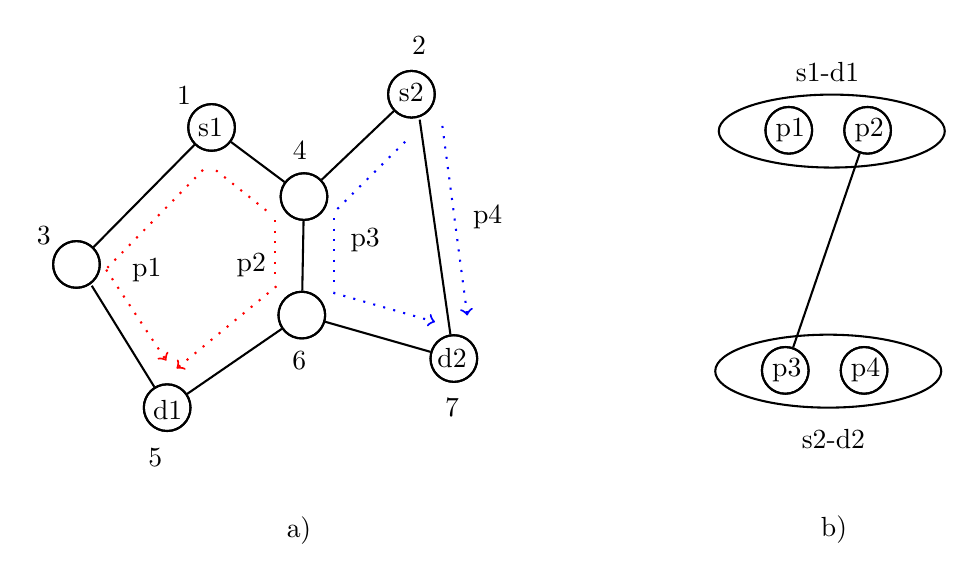
\begin{tikzpicture}
\pgftransformxscale{1.000000}
\pgftransformyscale{-1.000000}
\definecolor{dialinecolor}{rgb}{0.000000, 0.000000, 0.000000}
\pgfsetstrokecolor{dialinecolor}
\definecolor{dialinecolor}{rgb}{1.000000, 1.000000, 1.000000}
\pgfsetfillcolor{dialinecolor}
\pgfsetlinewidth{0.050000\du}
\pgfsetdash{}{0pt}
\pgfsetdash{}{0pt}
\pgfsetbuttcap
\pgfsetmiterjoin
\pgfsetlinewidth{0.050000\du}
\pgfsetbuttcap
\pgfsetmiterjoin
\pgfsetdash{}{0pt}
\definecolor{dialinecolor}{rgb}{1.000000, 1.000000, 1.000000}
\pgfsetfillcolor{dialinecolor}
\pgfpathellipse{\pgfpoint{14.562500\du}{15.212500\du}}{\pgfpoint{0.562500\du}{0\du}}{\pgfpoint{0\du}{0.562500\du}}
\pgfusepath{fill}
\definecolor{dialinecolor}{rgb}{0.000000, 0.000000, 0.000000}
\pgfsetstrokecolor{dialinecolor}
\pgfpathellipse{\pgfpoint{14.562500\du}{15.212500\du}}{\pgfpoint{0.562500\du}{0\du}}{\pgfpoint{0\du}{0.562500\du}}
\pgfusepath{stroke}
\pgfsetbuttcap
\pgfsetmiterjoin
\pgfsetdash{}{0pt}
\definecolor{dialinecolor}{rgb}{0.000000, 0.000000, 0.000000}
\pgfsetstrokecolor{dialinecolor}
\pgfpathellipse{\pgfpoint{14.562500\du}{15.212500\du}}{\pgfpoint{0.562500\du}{0\du}}{\pgfpoint{0\du}{0.562500\du}}
\pgfusepath{stroke}
\pgfsetlinewidth{0.050000\du}
\pgfsetdash{}{0pt}
\pgfsetdash{}{0pt}
\pgfsetbuttcap
\pgfsetmiterjoin
\pgfsetlinewidth{0.050000\du}
\pgfsetbuttcap
\pgfsetmiterjoin
\pgfsetdash{}{0pt}
\definecolor{dialinecolor}{rgb}{1.000000, 1.000000, 1.000000}
\pgfsetfillcolor{dialinecolor}
\pgfpathellipse{\pgfpoint{16.747500\du}{18.662500\du}}{\pgfpoint{0.562500\du}{0\du}}{\pgfpoint{0\du}{0.562500\du}}
\pgfusepath{fill}
\definecolor{dialinecolor}{rgb}{0.000000, 0.000000, 0.000000}
\pgfsetstrokecolor{dialinecolor}
\pgfpathellipse{\pgfpoint{16.747500\du}{18.662500\du}}{\pgfpoint{0.562500\du}{0\du}}{\pgfpoint{0\du}{0.562500\du}}
\pgfusepath{stroke}
\pgfsetbuttcap
\pgfsetmiterjoin
\pgfsetdash{}{0pt}
\definecolor{dialinecolor}{rgb}{0.000000, 0.000000, 0.000000}
\pgfsetstrokecolor{dialinecolor}
\pgfpathellipse{\pgfpoint{16.747500\du}{18.662500\du}}{\pgfpoint{0.562500\du}{0\du}}{\pgfpoint{0\du}{0.562500\du}}
\pgfusepath{stroke}
\pgfsetlinewidth{0.050000\du}
\pgfsetdash{}{0pt}
\pgfsetdash{}{0pt}
\pgfsetbuttcap
\pgfsetmiterjoin
\pgfsetlinewidth{0.050000\du}
\pgfsetbuttcap
\pgfsetmiterjoin
\pgfsetdash{}{0pt}
\definecolor{dialinecolor}{rgb}{1.000000, 1.000000, 1.000000}
\pgfsetfillcolor{dialinecolor}
\pgfpathellipse{\pgfpoint{22.632500\du}{11.112500\du}}{\pgfpoint{0.562500\du}{0\du}}{\pgfpoint{0\du}{0.562500\du}}
\pgfusepath{fill}
\definecolor{dialinecolor}{rgb}{0.000000, 0.000000, 0.000000}
\pgfsetstrokecolor{dialinecolor}
\pgfpathellipse{\pgfpoint{22.632500\du}{11.112500\du}}{\pgfpoint{0.562500\du}{0\du}}{\pgfpoint{0\du}{0.562500\du}}
\pgfusepath{stroke}
\pgfsetbuttcap
\pgfsetmiterjoin
\pgfsetdash{}{0pt}
\definecolor{dialinecolor}{rgb}{0.000000, 0.000000, 0.000000}
\pgfsetstrokecolor{dialinecolor}
\pgfpathellipse{\pgfpoint{22.632500\du}{11.112500\du}}{\pgfpoint{0.562500\du}{0\du}}{\pgfpoint{0\du}{0.562500\du}}
\pgfusepath{stroke}
\pgfsetlinewidth{0.050000\du}
\pgfsetdash{}{0pt}
\pgfsetdash{}{0pt}
\pgfsetbuttcap
\pgfsetmiterjoin
\pgfsetlinewidth{0.050000\du}
\pgfsetbuttcap
\pgfsetmiterjoin
\pgfsetdash{}{0pt}
\definecolor{dialinecolor}{rgb}{1.000000, 1.000000, 1.000000}
\pgfsetfillcolor{dialinecolor}
\pgfpathellipse{\pgfpoint{17.817500\du}{11.912500\du}}{\pgfpoint{0.562500\du}{0\du}}{\pgfpoint{0\du}{0.562500\du}}
\pgfusepath{fill}
\definecolor{dialinecolor}{rgb}{0.000000, 0.000000, 0.000000}
\pgfsetstrokecolor{dialinecolor}
\pgfpathellipse{\pgfpoint{17.817500\du}{11.912500\du}}{\pgfpoint{0.562500\du}{0\du}}{\pgfpoint{0\du}{0.562500\du}}
\pgfusepath{stroke}
\pgfsetbuttcap
\pgfsetmiterjoin
\pgfsetdash{}{0pt}
\definecolor{dialinecolor}{rgb}{0.000000, 0.000000, 0.000000}
\pgfsetstrokecolor{dialinecolor}
\pgfpathellipse{\pgfpoint{17.817500\du}{11.912500\du}}{\pgfpoint{0.562500\du}{0\du}}{\pgfpoint{0\du}{0.562500\du}}
\pgfusepath{stroke}
\pgfsetlinewidth{0.050000\du}
\pgfsetdash{}{0pt}
\pgfsetdash{}{0pt}
\pgfsetbuttcap
\pgfsetmiterjoin
\pgfsetlinewidth{0.050000\du}
\pgfsetbuttcap
\pgfsetmiterjoin
\pgfsetdash{}{0pt}
\definecolor{dialinecolor}{rgb}{1.000000, 1.000000, 1.000000}
\pgfsetfillcolor{dialinecolor}
\pgfpathellipse{\pgfpoint{20.043921\du}{13.577576\du}}{\pgfpoint{0.562500\du}{0\du}}{\pgfpoint{0\du}{0.562500\du}}
\pgfusepath{fill}
\definecolor{dialinecolor}{rgb}{0.000000, 0.000000, 0.000000}
\pgfsetstrokecolor{dialinecolor}
\pgfpathellipse{\pgfpoint{20.043921\du}{13.577576\du}}{\pgfpoint{0.562500\du}{0\du}}{\pgfpoint{0\du}{0.562500\du}}
\pgfusepath{stroke}
\pgfsetbuttcap
\pgfsetmiterjoin
\pgfsetdash{}{0pt}
\definecolor{dialinecolor}{rgb}{0.000000, 0.000000, 0.000000}
\pgfsetstrokecolor{dialinecolor}
\pgfpathellipse{\pgfpoint{20.043921\du}{13.577576\du}}{\pgfpoint{0.562500\du}{0\du}}{\pgfpoint{0\du}{0.562500\du}}
\pgfusepath{stroke}
\pgfsetlinewidth{0.050000\du}
\pgfsetdash{}{0pt}
\pgfsetdash{}{0pt}
\pgfsetbuttcap
\pgfsetmiterjoin
\pgfsetlinewidth{0.050000\du}
\pgfsetbuttcap
\pgfsetmiterjoin
\pgfsetdash{}{0pt}
\definecolor{dialinecolor}{rgb}{1.000000, 1.000000, 1.000000}
\pgfsetfillcolor{dialinecolor}
\pgfpathellipse{\pgfpoint{23.654200\du}{17.479200\du}}{\pgfpoint{0.562500\du}{0\du}}{\pgfpoint{0\du}{0.562500\du}}
\pgfusepath{fill}
\definecolor{dialinecolor}{rgb}{0.000000, 0.000000, 0.000000}
\pgfsetstrokecolor{dialinecolor}
\pgfpathellipse{\pgfpoint{23.654200\du}{17.479200\du}}{\pgfpoint{0.562500\du}{0\du}}{\pgfpoint{0\du}{0.562500\du}}
\pgfusepath{stroke}
\pgfsetbuttcap
\pgfsetmiterjoin
\pgfsetdash{}{0pt}
\definecolor{dialinecolor}{rgb}{0.000000, 0.000000, 0.000000}
\pgfsetstrokecolor{dialinecolor}
\pgfpathellipse{\pgfpoint{23.654200\du}{17.479200\du}}{\pgfpoint{0.562500\du}{0\du}}{\pgfpoint{0\du}{0.562500\du}}
\pgfusepath{stroke}
% setfont left to latex
\definecolor{dialinecolor}{rgb}{0.000000, 0.000000, 0.000000}
\pgfsetstrokecolor{dialinecolor}
\node[anchor=west] at (16.742500\du,11.145833\du){1};
% setfont left to latex
\definecolor{dialinecolor}{rgb}{0.000000, 0.000000, 0.000000}
\pgfsetstrokecolor{dialinecolor}
\node[anchor=west] at (22.399167\du,9.945833\du){2};
% setfont left to latex
\definecolor{dialinecolor}{rgb}{0.000000, 0.000000, 0.000000}
\pgfsetstrokecolor{dialinecolor}
\node[anchor=west] at (17.300000\du,10.250000\du){};
% setfont left to latex
\definecolor{dialinecolor}{rgb}{0.000000, 0.000000, 0.000000}
\pgfsetstrokecolor{dialinecolor}
\node[anchor=west] at (13.362500\du,14.529167\du){3};
% setfont left to latex
\definecolor{dialinecolor}{rgb}{0.000000, 0.000000, 0.000000}
\pgfsetstrokecolor{dialinecolor}
\node[anchor=west] at (19.531421\du,12.477576\du){4};
% setfont left to latex
\definecolor{dialinecolor}{rgb}{0.000000, 0.000000, 0.000000}
\pgfsetstrokecolor{dialinecolor}
\node[anchor=west] at (16.047500\du,19.862500\du){5};
\pgfsetlinewidth{0.050000\du}
\pgfsetdash{}{0pt}
\pgfsetdash{}{0pt}
\pgfsetbuttcap
{
\definecolor{dialinecolor}{rgb}{0.000000, 0.000000, 0.000000}
\pgfsetfillcolor{dialinecolor}
% was here!!!
\definecolor{dialinecolor}{rgb}{0.000000, 0.000000, 0.000000}
\pgfsetstrokecolor{dialinecolor}
\draw (17.407446\du,12.328223\du)--(14.972554\du,14.796777\du);
}
\pgfsetlinewidth{0.050000\du}
\pgfsetdash{}{0pt}
\pgfsetdash{}{0pt}
\pgfsetbuttcap
{
\definecolor{dialinecolor}{rgb}{0.000000, 0.000000, 0.000000}
\pgfsetfillcolor{dialinecolor}
% was here!!!
\definecolor{dialinecolor}{rgb}{0.000000, 0.000000, 0.000000}
\pgfsetstrokecolor{dialinecolor}
\draw (14.931300\du,15.725000\du)--(16.438666\du,18.162996\du);
}
\pgfsetlinewidth{0.050000\du}
\pgfsetdash{}{0pt}
\pgfsetdash{}{0pt}
\pgfsetbuttcap
{
\definecolor{dialinecolor}{rgb}{0.000000, 0.000000, 0.000000}
\pgfsetfillcolor{dialinecolor}
% was here!!!
\definecolor{dialinecolor}{rgb}{0.000000, 0.000000, 0.000000}
\pgfsetstrokecolor{dialinecolor}
\draw (18.287679\du,12.264133\du)--(19.573742\du,13.225942\du);
}
\pgfsetlinewidth{0.050000\du}
\pgfsetdash{}{0pt}
\pgfsetdash{}{0pt}
\pgfsetbuttcap
{
\definecolor{dialinecolor}{rgb}{0.000000, 0.000000, 0.000000}
\pgfsetfillcolor{dialinecolor}
% was here!!!
\definecolor{dialinecolor}{rgb}{0.000000, 0.000000, 0.000000}
\pgfsetstrokecolor{dialinecolor}
\draw (19.508435\du,16.764690\du)--(17.230624\du,18.330411\du);
}
\pgfsetlinewidth{0.050000\du}
\pgfsetdash{}{0pt}
\pgfsetdash{}{0pt}
\pgfsetbuttcap
{
\definecolor{dialinecolor}{rgb}{0.000000, 0.000000, 0.000000}
\pgfsetfillcolor{dialinecolor}
% was here!!!
\definecolor{dialinecolor}{rgb}{0.000000, 0.000000, 0.000000}
\pgfsetstrokecolor{dialinecolor}
\draw (22.207179\du,11.517528\du)--(20.469242\du,13.172547\du);
}
\pgfsetlinewidth{0.050000\du}
\pgfsetdash{}{0pt}
\pgfsetdash{}{0pt}
\pgfsetbuttcap
{
\definecolor{dialinecolor}{rgb}{0.000000, 0.000000, 0.000000}
\pgfsetfillcolor{dialinecolor}
% was here!!!
\definecolor{dialinecolor}{rgb}{0.000000, 0.000000, 0.000000}
\pgfsetstrokecolor{dialinecolor}
\draw (20.553117\du,16.593066\du)--(23.092643\du,17.318735\du);
}
\pgfsetlinewidth{0.050000\du}
\pgfsetdash{}{0pt}
\pgfsetdash{}{0pt}
\pgfsetbuttcap
{
\definecolor{dialinecolor}{rgb}{0.000000, 0.000000, 0.000000}
\pgfsetfillcolor{dialinecolor}
% was here!!!
\definecolor{dialinecolor}{rgb}{0.000000, 0.000000, 0.000000}
\pgfsetstrokecolor{dialinecolor}
\draw (22.831300\du,11.725000\du)--(23.571227\du,16.899004\du);
}
% setfont left to latex
\definecolor{dialinecolor}{rgb}{1.000000, 0.000000, 0.000000}
\pgfsetstrokecolor{dialinecolor}
\node[anchor=west] at (17.247900\du,11.908333\du){s1};
% setfont left to latex
\definecolor{dialinecolor}{rgb}{0.000000, 0.000000, 1.000000}
\pgfsetstrokecolor{dialinecolor}
\node[anchor=west] at (22.082500\du,11.062500\du){s2};
% setfont left to latex
\definecolor{dialinecolor}{rgb}{0.000000, 0.000000, 1.000000}
\pgfsetstrokecolor{dialinecolor}
\node[anchor=west] at (23.010400\du,17.475000\du){d2};
% setfont left to latex
\definecolor{dialinecolor}{rgb}{1.000000, 0.000000, 0.000000}
\pgfsetstrokecolor{dialinecolor}
\node[anchor=west] at (16.160400\du,18.708300\du){d1};
\pgfsetlinewidth{0.050000\du}
\pgfsetdash{{\pgflinewidth}{0.200000\du}}{0cm}
\pgfsetdash{{\pgflinewidth}{0.200000\du}}{0cm}
\pgfsetbuttcap
{
\definecolor{dialinecolor}{rgb}{1.000000, 0.000000, 0.000000}
\pgfsetfillcolor{dialinecolor}
% was here!!!
\definecolor{dialinecolor}{rgb}{1.000000, 0.000000, 0.000000}
\pgfsetstrokecolor{dialinecolor}
\draw (17.611544\du,12.934315\du)--(15.307430\du,15.292183\du);
}
\pgfsetlinewidth{0.050000\du}
\pgfsetdash{{\pgflinewidth}{0.200000\du}}{0cm}
\pgfsetdash{{\pgflinewidth}{0.200000\du}}{0cm}
\pgfsetbuttcap
{
\definecolor{dialinecolor}{rgb}{1.000000, 0.000000, 0.000000}
\pgfsetfillcolor{dialinecolor}
% was here!!!
\pgfsetarrowsend{to}
\definecolor{dialinecolor}{rgb}{1.000000, 0.000000, 0.000000}
\pgfsetstrokecolor{dialinecolor}
\draw (15.278092\du,15.338478\du)--(16.727660\du,17.530509\du);
}
\pgfsetlinewidth{0.050000\du}
\pgfsetdash{{\pgflinewidth}{0.200000\du}}{0cm}
\pgfsetdash{{\pgflinewidth}{0.200000\du}}{0cm}
\pgfsetbuttcap
{
\definecolor{dialinecolor}{rgb}{1.000000, 0.000000, 0.000000}
\pgfsetfillcolor{dialinecolor}
% was here!!!
\definecolor{dialinecolor}{rgb}{1.000000, 0.000000, 0.000000}
\pgfsetstrokecolor{dialinecolor}
\draw (17.925100\du,12.946573\du)--(19.267179\du,14.016979\du);
}
\pgfsetlinewidth{0.050000\du}
\pgfsetdash{{\pgflinewidth}{0.200000\du}}{0cm}
\pgfsetdash{{\pgflinewidth}{0.200000\du}}{0cm}
\pgfsetbuttcap
{
\definecolor{dialinecolor}{rgb}{1.000000, 0.000000, 0.000000}
\pgfsetfillcolor{dialinecolor}
% was here!!!
\pgfsetarrowsend{to}
\definecolor{dialinecolor}{rgb}{1.000000, 0.000000, 0.000000}
\pgfsetstrokecolor{dialinecolor}
\draw (19.379311\du,15.739035\du)--(16.975148\du,17.718934\du);
}
\pgfsetlinewidth{0.050000\du}
\pgfsetdash{{\pgflinewidth}{0.200000\du}}{0cm}
\pgfsetdash{{\pgflinewidth}{0.200000\du}}{0cm}
\pgfsetbuttcap
{
\definecolor{dialinecolor}{rgb}{0.000000, 0.000000, 1.000000}
\pgfsetfillcolor{dialinecolor}
% was here!!!
\definecolor{dialinecolor}{rgb}{0.000000, 0.000000, 1.000000}
\pgfsetstrokecolor{dialinecolor}
\draw (22.480196\du,12.254873\du)--(20.750100\du,13.971573\du);
}
\pgfsetlinewidth{0.050000\du}
\pgfsetdash{{\pgflinewidth}{0.200000\du}}{0cm}
\pgfsetdash{{\pgflinewidth}{0.200000\du}}{0cm}
\pgfsetbuttcap
{
\definecolor{dialinecolor}{rgb}{0.000000, 0.000000, 1.000000}
\pgfsetfillcolor{dialinecolor}
% was here!!!
\pgfsetarrowsend{to}
\definecolor{dialinecolor}{rgb}{0.000000, 0.000000, 1.000000}
\pgfsetstrokecolor{dialinecolor}
\draw (20.750100\du,15.896573\du)--(23.200100\du,16.596573\du);
}
\pgfsetlinewidth{0.050000\du}
\pgfsetdash{{\pgflinewidth}{0.200000\du}}{0cm}
\pgfsetdash{{\pgflinewidth}{0.200000\du}}{0cm}
\pgfsetbuttcap
{
\definecolor{dialinecolor}{rgb}{0.000000, 0.000000, 1.000000}
\pgfsetfillcolor{dialinecolor}
% was here!!!
\pgfsetarrowsend{to}
\definecolor{dialinecolor}{rgb}{0.000000, 0.000000, 1.000000}
\pgfsetstrokecolor{dialinecolor}
\draw (23.377100\du,11.875000\du)--(23.977100\du,16.441700\du);
}
\pgfsetlinewidth{0.050000\du}
\pgfsetdash{}{0pt}
\pgfsetdash{}{0pt}
\pgfsetbuttcap
{
\definecolor{dialinecolor}{rgb}{0.000000, 0.000000, 0.000000}
\pgfsetfillcolor{dialinecolor}
% was here!!!
\definecolor{dialinecolor}{rgb}{0.000000, 0.000000, 0.000000}
\pgfsetstrokecolor{dialinecolor}
\draw (31.827938\du,17.209561\du)--(33.430965\du,12.536023\du);
}
\pgfsetlinewidth{0.050000\du}
\pgfsetdash{}{0pt}
\pgfsetdash{}{0pt}
\definecolor{dialinecolor}{rgb}{0.000000, 0.000000, 0.000000}
\pgfsetstrokecolor{dialinecolor}
\pgfpathellipse{\pgfpoint{32.758022\du}{11.999695\du}}{\pgfpoint{2.722361\du}{0\du}}{\pgfpoint{0\du}{0.878858\du}}
\pgfusepath{stroke}
\pgfsetlinewidth{0.050000\du}
\pgfsetdash{}{0pt}
\pgfsetdash{}{0pt}
\pgfsetbuttcap
\pgfsetmiterjoin
\pgfsetlinewidth{0.050000\du}
\pgfsetbuttcap
\pgfsetmiterjoin
\pgfsetdash{}{0pt}
\definecolor{dialinecolor}{rgb}{0.000000, 0.000000, 0.000000}
\pgfsetstrokecolor{dialinecolor}
\pgfpathellipse{\pgfpoint{31.722712\du}{11.981129\du}}{\pgfpoint{0.562500\du}{0\du}}{\pgfpoint{0\du}{0.562500\du}}
\pgfusepath{stroke}
\pgfsetbuttcap
\pgfsetmiterjoin
\pgfsetdash{}{0pt}
\definecolor{dialinecolor}{rgb}{0.000000, 0.000000, 0.000000}
\pgfsetstrokecolor{dialinecolor}
\pgfpathellipse{\pgfpoint{31.722712\du}{11.981129\du}}{\pgfpoint{0.562500\du}{0\du}}{\pgfpoint{0\du}{0.562500\du}}
\pgfusepath{stroke}
\pgfsetlinewidth{0.050000\du}
\pgfsetdash{}{0pt}
\pgfsetdash{}{0pt}
\pgfsetbuttcap
\pgfsetmiterjoin
\pgfsetlinewidth{0.050000\du}
\pgfsetbuttcap
\pgfsetmiterjoin
\pgfsetdash{}{0pt}
\definecolor{dialinecolor}{rgb}{0.000000, 0.000000, 0.000000}
\pgfsetstrokecolor{dialinecolor}
\pgfpathellipse{\pgfpoint{33.621294\du}{11.981129\du}}{\pgfpoint{0.562500\du}{0\du}}{\pgfpoint{0\du}{0.562500\du}}
\pgfusepath{stroke}
\pgfsetbuttcap
\pgfsetmiterjoin
\pgfsetdash{}{0pt}
\definecolor{dialinecolor}{rgb}{0.000000, 0.000000, 0.000000}
\pgfsetstrokecolor{dialinecolor}
\pgfpathellipse{\pgfpoint{33.621294\du}{11.981129\du}}{\pgfpoint{0.562500\du}{0\du}}{\pgfpoint{0\du}{0.562500\du}}
\pgfusepath{stroke}
\pgfsetlinewidth{0.050000\du}
\pgfsetdash{}{0pt}
\pgfsetdash{}{0pt}
\definecolor{dialinecolor}{rgb}{0.000000, 0.000000, 0.000000}
\pgfsetstrokecolor{dialinecolor}
\pgfpathellipse{\pgfpoint{32.672918\du}{17.783021\du}}{\pgfpoint{2.722361\du}{0\du}}{\pgfpoint{0\du}{0.878858\du}}
\pgfusepath{stroke}
\pgfsetlinewidth{0.050000\du}
\pgfsetdash{}{0pt}
\pgfsetdash{}{0pt}
\pgfsetbuttcap
\pgfsetmiterjoin
\pgfsetlinewidth{0.050000\du}
\pgfsetbuttcap
\pgfsetmiterjoin
\pgfsetdash{}{0pt}
\definecolor{dialinecolor}{rgb}{1.000000, 1.000000, 1.000000}
\pgfsetfillcolor{dialinecolor}
\pgfpathellipse{\pgfpoint{31.637608\du}{17.764455\du}}{\pgfpoint{0.562500\du}{0\du}}{\pgfpoint{0\du}{0.562500\du}}
\pgfusepath{fill}
\definecolor{dialinecolor}{rgb}{0.000000, 0.000000, 0.000000}
\pgfsetstrokecolor{dialinecolor}
\pgfpathellipse{\pgfpoint{31.637608\du}{17.764455\du}}{\pgfpoint{0.562500\du}{0\du}}{\pgfpoint{0\du}{0.562500\du}}
\pgfusepath{stroke}
\pgfsetbuttcap
\pgfsetmiterjoin
\pgfsetdash{}{0pt}
\definecolor{dialinecolor}{rgb}{0.000000, 0.000000, 0.000000}
\pgfsetstrokecolor{dialinecolor}
\pgfpathellipse{\pgfpoint{31.637608\du}{17.764455\du}}{\pgfpoint{0.562500\du}{0\du}}{\pgfpoint{0\du}{0.562500\du}}
\pgfusepath{stroke}
\pgfsetlinewidth{0.050000\du}
\pgfsetdash{}{0pt}
\pgfsetdash{}{0pt}
\pgfsetbuttcap
\pgfsetmiterjoin
\pgfsetlinewidth{0.050000\du}
\pgfsetbuttcap
\pgfsetmiterjoin
\pgfsetdash{}{0pt}
\definecolor{dialinecolor}{rgb}{1.000000, 1.000000, 1.000000}
\pgfsetfillcolor{dialinecolor}
\pgfpathellipse{\pgfpoint{33.536190\du}{17.764455\du}}{\pgfpoint{0.562500\du}{0\du}}{\pgfpoint{0\du}{0.562500\du}}
\pgfusepath{fill}
\definecolor{dialinecolor}{rgb}{0.000000, 0.000000, 0.000000}
\pgfsetstrokecolor{dialinecolor}
\pgfpathellipse{\pgfpoint{33.536190\du}{17.764455\du}}{\pgfpoint{0.562500\du}{0\du}}{\pgfpoint{0\du}{0.562500\du}}
\pgfusepath{stroke}
\pgfsetbuttcap
\pgfsetmiterjoin
\pgfsetdash{}{0pt}
\definecolor{dialinecolor}{rgb}{0.000000, 0.000000, 0.000000}
\pgfsetstrokecolor{dialinecolor}
\pgfpathellipse{\pgfpoint{33.536190\du}{17.764455\du}}{\pgfpoint{0.562500\du}{0\du}}{\pgfpoint{0\du}{0.562500\du}}
\pgfusepath{stroke}
% setfont left to latex
\definecolor{dialinecolor}{rgb}{1.000000, 0.000000, 0.000000}
\pgfsetstrokecolor{dialinecolor}
\node[anchor=west] at (31.647614\du,10.565507\du){s1-d1};
% setfont left to latex
\definecolor{dialinecolor}{rgb}{0.000000, 0.000000, 1.000000}
\pgfsetstrokecolor{dialinecolor}
\node[anchor=west] at (31.789035\du,19.404342\du){s2-d2};
% setfont left to latex
\definecolor{dialinecolor}{rgb}{0.000000, 0.000000, 0.000000}
\pgfsetstrokecolor{dialinecolor}
\node[anchor=west] at (16.055909\du,15.409188\du){};
% setfont left to latex
\definecolor{dialinecolor}{rgb}{1.000000, 0.000000, 0.000000}
\pgfsetstrokecolor{dialinecolor}
\node[anchor=west] at (15.658422\du,15.347056\du){p1};
% setfont left to latex
\definecolor{dialinecolor}{rgb}{1.000000, 0.000000, 0.000000}
\pgfsetstrokecolor{dialinecolor}
\node[anchor=west] at (18.176189\du,15.225610\du){p2};
% setfont left to latex
\definecolor{dialinecolor}{rgb}{0.000000, 0.000000, 1.000000}
\pgfsetstrokecolor{dialinecolor}
\node[anchor=west] at (20.917789\du,14.637437\du){p3};
% setfont left to latex
\definecolor{dialinecolor}{rgb}{0.000000, 0.000000, 1.000000}
\pgfsetstrokecolor{dialinecolor}
\node[anchor=west] at (23.869439\du,14.065685\du){p4};
% setfont left to latex
\definecolor{dialinecolor}{rgb}{1.000000, 0.000000, 0.000000}
\pgfsetstrokecolor{dialinecolor}
\node[anchor=west] at (31.160212\du,11.981129\du){p1};
% setfont left to latex
\definecolor{dialinecolor}{rgb}{1.000000, 0.000000, 0.000000}
\pgfsetstrokecolor{dialinecolor}
\node[anchor=west] at (33.058794\du,11.981129\du){p2};
% setfont left to latex
\definecolor{dialinecolor}{rgb}{0.000000, 0.000000, 1.000000}
\pgfsetstrokecolor{dialinecolor}
\node[anchor=west] at (31.075108\du,17.764455\du){p3};
% setfont left to latex
\definecolor{dialinecolor}{rgb}{0.000000, 0.000000, 1.000000}
\pgfsetstrokecolor{dialinecolor}
\node[anchor=west] at (32.973690\du,17.764455\du){p4};
% setfont left to latex
\definecolor{dialinecolor}{rgb}{0.000000, 0.000000, 0.000000}
\pgfsetstrokecolor{dialinecolor}
\node[anchor=west] at (19.379311\du,21.631728\du){a)};
% setfont left to latex
\definecolor{dialinecolor}{rgb}{0.000000, 0.000000, 0.000000}
\pgfsetstrokecolor{dialinecolor}
\node[anchor=west] at (32.248654\du,21.596373\du){b)};
\pgfsetlinewidth{0.050000\du}
\pgfsetdash{}{0pt}
\pgfsetdash{}{0pt}
\pgfsetbuttcap
\pgfsetmiterjoin
\pgfsetlinewidth{0.050000\du}
\pgfsetbuttcap
\pgfsetmiterjoin
\pgfsetdash{}{0pt}
\definecolor{dialinecolor}{rgb}{1.000000, 1.000000, 1.000000}
\pgfsetfillcolor{dialinecolor}
\pgfpathellipse{\pgfpoint{19.991560\du}{16.432601\du}}{\pgfpoint{0.562500\du}{0\du}}{\pgfpoint{0\du}{0.562500\du}}
\pgfusepath{fill}
\definecolor{dialinecolor}{rgb}{0.000000, 0.000000, 0.000000}
\pgfsetstrokecolor{dialinecolor}
\pgfpathellipse{\pgfpoint{19.991560\du}{16.432601\du}}{\pgfpoint{0.562500\du}{0\du}}{\pgfpoint{0\du}{0.562500\du}}
\pgfusepath{stroke}
\pgfsetbuttcap
\pgfsetmiterjoin
\pgfsetdash{}{0pt}
\definecolor{dialinecolor}{rgb}{0.000000, 0.000000, 0.000000}
\pgfsetstrokecolor{dialinecolor}
\pgfpathellipse{\pgfpoint{19.991560\du}{16.432601\du}}{\pgfpoint{0.562500\du}{0\du}}{\pgfpoint{0\du}{0.562500\du}}
\pgfusepath{stroke}
\pgfsetlinewidth{0.050000\du}
\pgfsetdash{}{0pt}
\pgfsetdash{}{0pt}
\pgfsetbuttcap
{
\definecolor{dialinecolor}{rgb}{0.000000, 0.000000, 0.000000}
\pgfsetfillcolor{dialinecolor}
% was here!!!
\definecolor{dialinecolor}{rgb}{0.000000, 0.000000, 0.000000}
\pgfsetstrokecolor{dialinecolor}
\draw (20.033158\du,14.164473\du)--(20.002323\du,15.845704\du);
}
% setfont left to latex
\definecolor{dialinecolor}{rgb}{0.000000, 0.000000, 0.000000}
\pgfsetstrokecolor{dialinecolor}
\node[anchor=west] at (19.516889\du,17.539251\du){6};
% setfont left to latex
\definecolor{dialinecolor}{rgb}{0.000000, 0.000000, 0.000000}
\pgfsetstrokecolor{dialinecolor}
\node[anchor=west] at (23.194581\du,18.664555\du){7};
\pgfsetlinewidth{0.050000\du}
\pgfsetdash{{\pgflinewidth}{0.200000\du}}{0cm}
\pgfsetdash{{\pgflinewidth}{0.200000\du}}{0cm}
\pgfsetbuttcap
{
\definecolor{dialinecolor}{rgb}{1.000000, 0.000000, 0.000000}
\pgfsetfillcolor{dialinecolor}
% was here!!!
\definecolor{dialinecolor}{rgb}{1.000000, 0.000000, 0.000000}
\pgfsetstrokecolor{dialinecolor}
\draw (19.343956\du,14.148045\du)--(19.343956\du,15.632969\du);
}
\pgfsetlinewidth{0.050000\du}
\pgfsetdash{{\pgflinewidth}{0.200000\du}}{0cm}
\pgfsetdash{{\pgflinewidth}{0.200000\du}}{0cm}
\pgfsetbuttcap
{
\definecolor{dialinecolor}{rgb}{0.000000, 0.000000, 1.000000}
\pgfsetfillcolor{dialinecolor}
% was here!!!
\definecolor{dialinecolor}{rgb}{0.000000, 0.000000, 1.000000}
\pgfsetstrokecolor{dialinecolor}
\draw (20.775100\du,14.096573\du)--(20.775100\du,15.846573\du);
}
\end{tikzpicture}

\caption{a) A graph with two source-destination pairs and two paths each. Since paths p2 and p3 share edge \{4,6\}, they are not allowed to use the same wavelength and therefore the corresponding nodes are adjacent in b) the resulting PCP.}
\label{pd:transformation}
\end{figure}
\end{center}


\section{Problem Complexity}

The decision variant of VCP asks for whether a graph can be colored within $k$ colors or not. For $k=2$ the answer can be computed in linear time by checking if the graph is bipartite. For $k\geq 3$, a certificate for a decision can only be given by a valid coloring. In chapter \ref{ch:prelim} it has been stated that the decision variant of VCP belongs to the class $\mathcal{NP}$. It has been proven in the early 1970s by Cook and Levin, that any problem in $\mathcal{NP}$ can be reduced to SAT. In complexity theory, SAT is one the most prominent NPOs in $\mathcal{NP}$ and it is widely assumed that there does not exist an algorithm that solves it exactly in polynomial time. This assumption is closely linked to the question $\mathcal{P} \neq \mathcal{NP}$.

\begin{definition}[SAT]
Given a set of clauses $C_1, \ldots , C_k$ in CNF over a set of variables $X = \{x_1,\ldots,x_n\}$, the SAT problem asks if there exist a satisfying assignment.
\end{definition}

\begin{theorem}[Cook Levin]
Any problem in $\mathcal{NP}$ can be reduced in polynomial time by a deterministic Touring machine to SAT.
\end{theorem}

Generating a $k$-coloring of a graph $G=(V,E)$ can be reduced to SAT as follows: For each possible node-color assignment, introduce a boolean variable $x_{vc}, v\in V, c\in \{1,\ldots ,k\}$. Considering the following formulas:
\begin{align}
\bigvee_{1\leq c \leq k}p_{vc} && (v\in V)\\
\neg (p_{vc} \wedge p_{vd}) 		&& (v\in V, 1 \leq i < j \leq k),\\
\neg (p_{vc} \wedge p_{wc})		&& (\{v,w\}\in E, 1 \leq i \leq k).
\end{align}

Finding an assignment satisfying these formulas is a one-to-one correspondence to finding a $k$-coloring of graph $G$.\\

When PCP is decomposed into two phases -- the node selection phase and the coloring phase -- it becomes clear that the coloring phase is equivalent to VCP, therefore $VCP \leq_P PCP$ holds. Li and Simha show in \cite{li-00} another way to reduce PCP to VCP.

\begin{theorem}
PCP is $\mathcal{NP}$-hard.
\end{theorem}

Similarly, min-RWA can be decomposed into two phases, where the assignment phase is equivalent to PCP, as shown in section \ref{sec:minrwa}. A proof of $\mathcal{NP}$-hardness has been provided by Erlebach and Jansen in \cite{erlebach-01}.

\begin{theorem}
min-RWA is $\mathcal{NP}$-hard.
\end{theorem}